\chapter{Minimum Number of Sensors to Ensure Observability of Physical Systems: Case Studies}
\label{cha:ch4}

Advances in wearable technology allow us to measure all sorts of physiological signals. Fitbit is probably the most familiar to the public in general. It measures data such as the number of steps per day, quality of sleep, steps climbed, and other personal metrics; and  Emotiv is a company that  develops brain-computer interfaces based on electroencephalography (EEG) technology. Nonetheless, these and other technologies are still in their infancy, and far from allowing to predict a cardiac arrest or the beginning of an epileptic seizure. The benefits generated by such capability are expected to revolutionize healthcare, in the sense that it will allow an impairment with a smartphone via wireless or bluetooth, capable of performing an emergency call, or stimulate locally certain points of the human body to mitigate the effects that follow each occurrences. 

Towards that auspicious future, we propose to explore a class of models that will enable the characterization of certain physiological signal dynamics, and allow us to retrieve the overall dynamics associated with certain technologies by only considering a subset of its signals. These models rely on the assumption that acquired signals of the same physiological phenomena have \textit{spatial-temporal properties} that can be captured by the model. This is the case for the electrocardiogram (ECG) signal that records the electrical voltages generated by the heart over a period of time, using electrodes placed across the patient's body: limbs and chest. Commonly, there are between twelve and sixteen ECG electrodes placed on the surface of the patient's body. These sensors capture the potential differences between electrodes that arise from heart-muscle depolarization during each cardiac cycle, measured from different angles in a frame whose heart sets the origin~\cite{hall2015guyton}. This emphasizes the \textit{spatial} and \textit{temporal interdependence} between physiological processes. Further, Fitbit sensor matches one of the leads locations, so one could wonder if it would suffice to predict abnormal cardiac activity, see Figure~\ref{fig:fitbit}. 

\begin{figure}[htb]
\centering
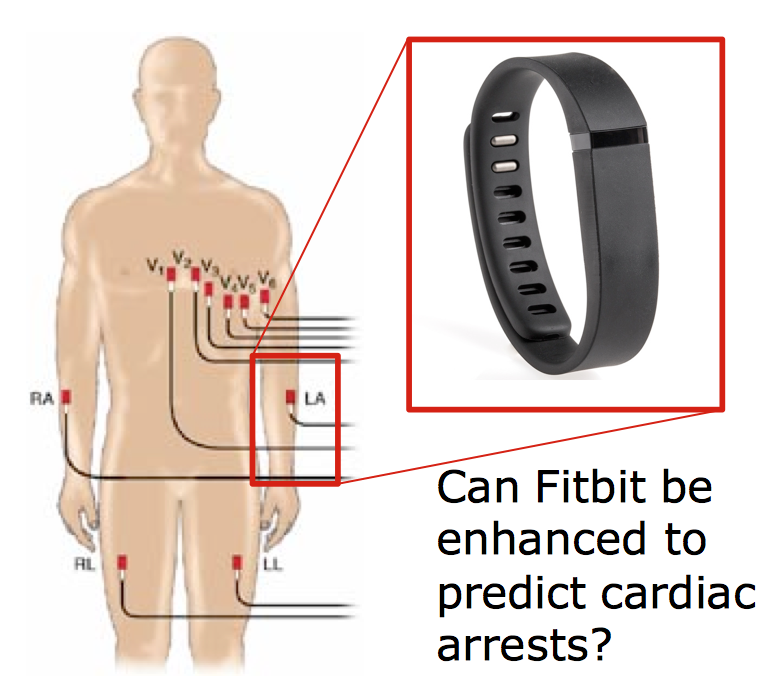
\includegraphics[width=0.50\columnwidth]{fitbit.png}
\caption{\textbf{Can the Fitbit sensor be used to retrieve the overall activity of the remaining sensors, hence, assess if one is about to have a cardiac arrest?}}\label{fig:fitbit}
\vskip -2mm
\end{figure}  

Similarly, the EEG sensors measure electrical potentials (brain waves) resulting from ionic current within the neurons of the brain. Due to the nature of the electrodes used, different sensors may collect data associated with the same activity, and, thus, capturing \textit{interdependent temporal} and \textit{spatial} signals. The frequency of the brain waves recorded from the surface of the scalp can range from once per few seconds to more than 50Hz. The aspect of these waves is dependent on the activity of the correspondent cerebral cortex being acquired, and they can change drastically between states of wakefullness, sleep, coma or in brain diseases such as epilepsy~\cite{hall2015guyton}. Finally,  an electromyography (EMG) signal detects the electrical potential generated by the skeletal muscle cells when these cells are electrically or neurologically activated, hence, resulting in a technique for evaluating and recording the electrical activity produced by skeletal muscles. These signals can then contain dynamical fingerprints that are associated with a configuration of muscle activation, leading to the execution of a specific task. Once again, due to the interdependence of the different biological systems (muscles) in the human body, it is easy to understand that the \textit{spatial} and \textit{temporal dependence} is present. Furthermore, these signals can be analyzed to detect and predict medical abnormalities, activation level, or recruitment order, or to analyze the biomechanics of human or animal movement. 

Unlike current mathematical modeling approaches that rely on memoryless assumptions, the statistical analysis of physiological processes (ECG, EEG, blood glucose) demonstrates that they possess significant degree of long-range memory and fractality. In particular, numerous recent studies show that physiological processes can be more accurately modeled via \emph{fractal order dynamical systems}~\cite{moon1992chaotic,piramideCortexFractal,surveyFractalNeuro,ecgFractal,Thurner2003511}.  Nonetheless, these efforts have either only demonstrated that the statistics of the physiological dynamics is of fractal nature (e.g., the autocorrelation function or the power spectrum exhibit a power law behavior) or only accounted for the temporal dependence of the signals (e.g., demonstrating that there is some form of persistence in time between changes in the magnitude of the physiological process). Subsequently, the spatial dependence existing between various physiological processes cannot be leveraged to obtain information about the signals that are not being directly measured. 

To overcome these limitations, we propose to use \textbf{coupled discrete-time fractal order dynamical systems} (CDFODS) to capture the spatial-temporal characteristics existing between physiological processes. Further, if we aim to retrieve the state of the system from the measurements alone, commonly referred to as \emph{static observability},  the solvability of a set of $p$ measurements equations to recover an $n-$dimensional parameter is required, hence, requiring at least as many measurements as the number of unknowns, $p\ge n$, in general. In addition, if the processes are not spatially dependent, when the sensing technology only accesses a state variable at any given time, then such conditions are not possible to satisfy.  Subsequently, this model allows us to retrieve all its states from the collected data obtained from a small subcollection and the model. This property is commonly referred to as \emph{observability} of the system, and the system (i.e., dynamics and sensing capabilities) that possesses it are referred to as being \emph{observable}~\cite{fracOrderdiscrete} -- see Section~\ref{prelim} for details. Furthermore, in this paper, we propose to extend the use of submodularity tools to find the minimum number of sensors in the CDFODS context that, to the best of our knowledge, has not yet been previously explored. 

Submodular functions are used across multiple fields of science, for instance, mathematics, economics,  circuit theory, operation research and machine learning~\cite{BachSurvey,Edmonds,Lovasz1983,Schrijver}. In particular, examples of machine learning applications include static sensor selection~\cite{KrauseGuestrinInfoGather,KrauseGuestrinSensorPlace} where a dynamic model is not explicitly considered; natural language processing~\cite{kirchhoff}; robotics applications~\cite{atanasov2015a,MeliouKGH07}; and  spatio-temporal processes modeled as linear-time-invariant models under uncertainty~\cite{aiStats}, just to name a few.  The problem of determining the minimum number of sensors to ensure observability in linear-time invariant systems has been explored in~\cite{MinControlProb}, and its optimal solutions in~\cite{PequitoJ4}. In addition, we notice that the previous solutions~\cite{MinControlProb,PequitoJ4} considered the continuous-time integer (non-fractional) order systems. It is also important to notice that although~\cite{MinControlProb,PequitoJ4} propose approximations that resemble the greedy algorithms known to approximate those whose objective are given by a submodular function,  they do not explicitly use these notions as we propose in this paper. 

The contributions of this paper are fourfold: (i) we explain how to cast the evolution of several spatial-temporal-related physiological signals into a CDFODS framework; (ii) we show that the problem of determining the minimum number of sensors required to ensure observability of CDFODS is NP-hard; (iii) we propose to use submodularity theory to approximate the results, which yields optimality guarantees; and  (iv) we show its application in the context of three physiological signals, i.e., EEG, ECG and EMG.

The remaining of the paper is organized as follows: Section~\ref{probStat} introduces the CDFODS and the mathematical formulation of the problem to determine the minimum number of sensors to obtain an observable system. In Section~\ref{prelim}, we revisit some of the properties of the CDFODS and submodularity theory. The theoretical  results of this paper are presented in Section~\ref{mainResults}, whereas in Section~\ref{illustExam} we study several applications of the proposed framework.


\section{Problem Statement}\label{probStat}
Consider a model dynamics described by a linear discrete-time fractional-order system as follows


%\begin{equation}
%\Delta^{\boldsymbol{\alpha}}x_{k+1}=\left[ \begin{array}{c}
%\Delta^{\alpha_1} x^1_{k+1}\\
%\Delta^{\alpha_2} x^2_{k+1}\\
%\vdots\\
%\Delta^{\alpha_n} x^n_{k+1}
%\end{array}
%\right]=\sum\limits_{j=0}^{k+1}A_j x_{k},\label{fracDyn}
%\end{equation}


\begin{equation}
\label{fracDyn}
\left[ \begin{array}{cccc}
D^{\alpha_1}&&&\\
%&D^{\alpha_2}&&\\
&&\ddots &\\
&&& D^{\alpha_n}
\end{array}
\right]x[k+1]=Ax[k],  
\end{equation}
where $k=0,1,\ldots, T$; $\alpha_i\in\mathbb{R}^{+}$ for $i=1,\ldots,n$; and $D^{\alpha_i}$ is the discretized fractional-order operator~\cite{fracOrderdiscrete}, and $x[0]=x_0\in\mathbb{R}^n$ the initial condition. Further, for brevity, we refer to the dynamics in~\eqref{fracDyn} as $\mathcal F(A;\boldsymbol{\alpha},K)$, where $\boldsymbol{\alpha}=(\alpha_1,\ldots, \alpha_n)$. In addition, assume that a collection of sensors is deployed to collect data about the state of the system. If a sensor is able to capture a linear combination of state variables, then the collection of sensors measurements can be represented as follows:
\begin{equation}
y[k]=Cx[k],
\label{outputGenericDiscrete}
\end{equation}
where $C$ is a matrix with appropriate dimensions encoding the linear combination. In the static case, i.e., when we aim to retrieve the state of the system from the measurements alone, (static) observability requires the solvability of a set of $p$ measurements equations to recover an $n-$dimensional parameter, hence, requiring at least as many measurements as the number of unknowns, $p\ge n$, in general. Alternatively, as often occurs in several setups, the sensor captures only a state variable (instead of a linear combination of these), i.e., the collection of measurements is given by
\begin{equation}
y[k]=\mathbb{I}_n^{\mathcal J}x[k],
\label{outputDiscrete}
\end{equation}
where $\mathcal J$ denotes the indices of the state  variables being measured, and $\mathbb{I}^{\mathcal J}_{n}$ denotes the matrix that consists of the rows of the identity matrix with indices in $\mathcal J$. Hence, no solution exists that retrieves the state variables that are not being measured, when only the collection of measurements is considered.  To overcome the two issues mentioned, we propose to  consider the model that captures the spatial-temporal relationship between the state variables that together with the measurements will enable the retrieval of the state. A system $\mathcal F(A;\boldsymbol{\alpha},K)$ and a collection of measurements~\eqref{outputDiscrete} is said to be (dynamically) \emph{observable} at time $k=0$ if and only if there exists some $T$ such that the state $x_0$ can be uniquely determined from the knowledge of $y_k$ and $\mathcal F(A;\boldsymbol{\alpha},K)$. Subsequently, the goal of this paper is to determine the minimum $\mathcal J$ in~\eqref{outputDiscrete} that, together with $\mathcal F(A;\boldsymbol{\alpha},K)$, ensures observability of the system at time $k=0$. We have the following problem:

  

\textit{Minimum Sensor Placement Problem}


Given $\mathcal F(A;\boldsymbol{\alpha},K)$,  determine the minimum number of dedicated sensors $\mathcal J$  such that
\begin{equation}
\begin{array}{cc}
\arg\min\limits_{\mathcal J\subset \{1,\ldots,n\}} & |\mathcal J|\\
\text{s.t.} & (\mathcal F(A;\boldsymbol{\alpha},K),\mathbb{I}_n^{\mathcal J}) \text{ is observable.}
\end{array}
\label{optProbP2}
\end{equation}
\hfill $\circ$

\begin{figure}[htb]
\centering
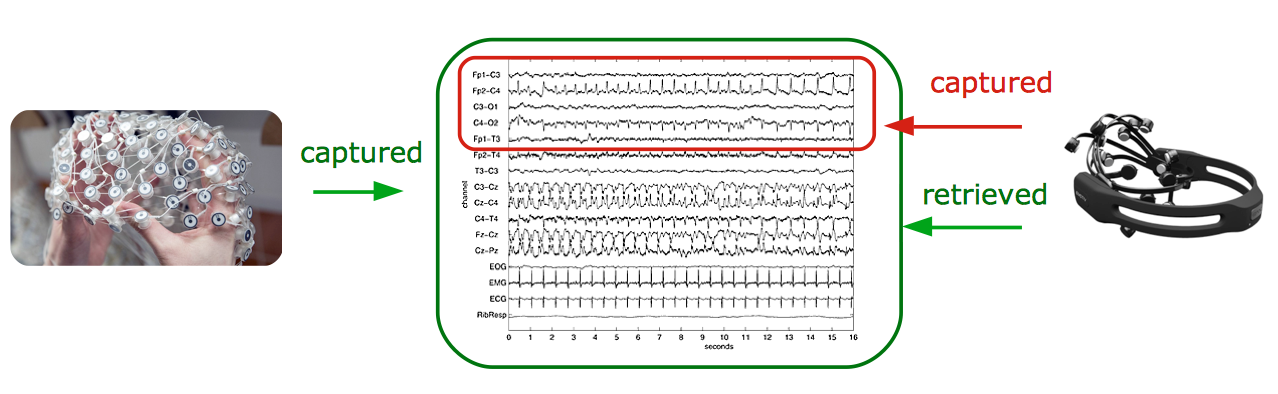
\includegraphics[width=1\columnwidth]{eegCapRec.png}
\caption{\textbf{Are both technologies equivalent?}}\label{fig:EEGCapRec}
\end{figure}

Figure~\ref{fig:EEGCapRec} illustrates one possible application of this problem, i.e., determine if a subcollection of sensors allow to retrieve the overall evolution of  EEG signals. In particular, determining the smallest collection of such sensors will lead to the development of energy efficient EEG wearables.





\section{CDFODS Observability and Submodularity}\label{prelim}

In this section, we first review  some properties of the CDFODS and the characterization of the feasibility space of~\eqref{optProbP2}, followed by a brief recap of submodularity properties. The closed-form to~\eqref{fracDyn} is described as follows.

\begin{lemma}[\cite{fracOrderdiscrete,fracOrderdiscreteJournal}]
The solution to~\eqref{fracDyn} is given by:
\begin{equation}
x[{k+1}]=G_{k+1}x[0],
\label{fracDynSol}
\end{equation}
\noindent where
\[
G_k=\left\{\begin{array}{cl}
\mathbb{I} & \text{for } k=0,\\
\sum\limits_{j=0}^{k-1}A_jG_{k-1-j}& \text{for } k\ge 1,
\end{array}\right.
\]

with $A_0=A$ and $A_j=\text{diag}(${\small$- (-1)^{j+1} \binom{\alpha_1}{j+1},\ldots,$ \\
$- (-1)^{j+1} \binom{\alpha_n}{j+1}$}$)$. Please note that $\alpha$ is a non-integer number and the term $\binom{\alpha}{j} = \frac{\Gamma(\alpha+1)}{\Gamma(j+1)\Gamma(\alpha-j+1)}$ is expressed via the Gamma function: $\Gamma (x) = \int_{0}^{\infty} t^{x-1}e^{-t}dt$ \cite{Baleanu}.\label{LemmaClosedForm}
\hfill $\diamond$
\end{lemma}

Subsequently, consider a sequence of measurements of the closed-form described in Lemma~\ref{LemmaClosedForm}, i.e.,
\begin{align*}
y[1]=Cx[1]=CG_0& x[0], \  y[2]=Cx[2]=CG_1x[0], \notag \\
 &\ldots, \ y[K]=Cx[K]=CG_{K-1}x[0].\notag
\end{align*}

We can rewrite it as
\begin{equation}
y_{0:K}=\underbrace{[(CG_0)^{\intercal} \ (CG_1)^{\intercal} \ \ldots \ (CG_{k-1})^{\intercal}]^{\intercal}}_{\mathcal O_k(\mathcal F(A;\mathbf{\alpha},K),C)}x[0],
\label{evolMeasurements}
\end{equation}
where $y_{0:K}=[y^\intercal_0 \  y^\intercal_1 \ \cdots \ y^\intercal_K]^\intercal$, and the matrix $\mathcal O_k(\mathcal F(A;\mathbf{\alpha},K),C)$ is commonly referred to as \emph{observability matrix}. In order to retrieve $x[0]$, we can first premultiply both hand sides of~\eqref{evolMeasurements} by $\mathcal O^{\intercal}\equiv\mathcal O_k(\mathcal F(A;\mathbf{\alpha},k),C)$, which leads to
\[
\mathcal O^{\intercal}y_{0:K}=\mathcal O^{\intercal}\mathcal Ox[0].
\]
Thus, if $\mathcal O^{\intercal}\mathcal O$ is invertible, then we obtain a closed-form solution to $x[0]$, i.e., 
\begin{equation}
x[0]=(\mathcal O^{\intercal}\mathcal O)^{-1}\mathcal O^{\intercal}y_{0:K}.\label{retrieveDynFracEq}
\end{equation}
As a consequence, we obtain the following results:




\begin{theorem}[\cite{fracOrderdiscrete,fracOrderdiscreteJournal}]
The system described by \eqref{fracDyn} and \eqref{outputGenericDiscrete}  is observable if and only if there exists a finite time $K$ such that $\text{rank } (\mathcal O_K(\mathcal F(A;\mathbf{\alpha},K),C))=n$. \hfill $\diamond$
\label{observabilityDynFrac}
\end{theorem}





\begin{theorem}[\cite{fracOrderdiscrete,fracOrderdiscreteJournal}]
If the system described by \eqref{fracDyn} and \eqref{outputGenericDiscrete}  is observable, then the initial state $x_0$ can be retrieved as in~\eqref{retrieveDynFracEq}.
\hfill $\diamond$
\label{retrieveDynFrac}
\end{theorem}

\begin{remark}
Due to the nature of Theorem~\ref{observabilityDynFrac}, it may occur that a specific set of measurements do not yield observability of a given time $K$. Notwithstanding, it is possible that there exits  $K'>K$ that for the same collection of sensors  such that Theorem~\ref{observabilityDynFrac} holds. In other words, observability implicit considers the tradeoffs between how much data is collected (with the same set of measurements), in particular, the  time allowed to collect data, and the number of sensors  acquiring it. \hfill $\diamond$
\end{remark}


In section 4, we show how the aforementioned characterization of the feasibility space of~\eqref{optProbP2} can be used to obtain its solution. Briefly, we will use a submodular approach. 

Given a finite set $\mathcal V$ with $n$ objects, i.e., $|\mathcal V|=n$, we can define a function $f:2^{\mathcal V}\rightarrow \mathbb{R}^+$ that associates a positive scalar with each subset of $\mathcal V$. This function is said to be \emph{submodular} if it satisfies the so-called \emph{diminishing returns} property, i.e., for all $\mathcal X\subset \mathcal Y$ and $v\notin \mathcal Y$, we must have: $$f(\mathcal X\cup \{v\})-f(\mathcal X)\ge f(\mathcal Y\cup \{v\})-f(\mathcal Y).$$ In other words, the increment by considering a new element in a smaller sized set is at least as high as adding it to a superset of the latter. When $f$ is submodular, one can use greedy algorithms that yield approximate solutions that are at most $33\%$ worse than the optimal solution~\cite{Nemhauser}. These approximation guarantee does not depend on the size of $\mathcal V$ and it provides a worst case scenario that is often not attained; in addition, some improved guarantees are available when submodular functions have additional properties, see~\cite{LinBilmes} for details.

\section{Minimum Sensor Placement}\label{mainResults}

In this section, we present the main results of this paper. More precisely, in Theorem~\ref{complexity} we show our problem to be NP-hard. Notwithstanding, we present an heuristic  Algorithm~\ref{algorithm1} that has polynomial computational complexity, and approximates the original problem with some optimality guarantees, see Theorem~\ref{algorithmApproxResult}. 



\begin{theorem}
The minimum sensor placement problem for CDFODS~\eqref{optProbP2} is NP-hard.\hfill $\diamond$
\label{complexity}
\end{theorem}

\textbf{Proof: }
The proof follows by noticing that there exists a set of coefficients $\mathbf{\alpha}$ that leads to $A_j=\mathbb{I}_n$ for $j=1,\ldots,K$. Therefore,~\eqref{optProbP2} reduces to a linear time-invariant system, and the problem reduces to the minimum observability problem for linear-time invariant systems presented in~\cite{MinControlProb}, that is NP-hard. Thus, because~\eqref{optProbP2} contains (as subclass of problems) one that is NP-hard, it follows that~\eqref{optProbP2} is also NP-hard.\hfill $\blacksquare$






\begin{algorithm}[tb]
   \caption{Heuristic Algorithm to~\eqref{optProbP2}}
   \label{algorithm1}
\begin{algorithmic}
   \STATE {\bfseries Input:} CDFODS $\mathcal F(A;\mathbf{\alpha},K)$;
      \STATE {\bfseries Output:} $\mathcal J^*$  that is an approximate solution to~\eqref{optProbP2};
      \vspace{0.2cm}
      {
   \STATE Initialize $ \mathcal J^*=\emptyset $; 
   \REPEAT
   \STATE Initialize $\Delta r^* = 0$;
   \STATE $r_{0}=\text{rank}(\mathcal O_k(\mathcal F(A;\mathbf{\alpha},K),\mathbb{I}_n^{\mathcal J^*}))$;
   \FOR{$i=1$ {\bfseries to} $n$}
   \STATE $\mathcal J'= \mathcal J^* \cup \{i\}$;
   \STATE $\Delta r(i)=\text{rank}(\mathcal O_k(\mathcal F(A;\mathbf{\alpha},K),\mathbb{I}_n^{\mathcal J'}))-r_{0}$;
   \IF{$\Delta r(i) > \Delta r^* $} 
   \STATE $\Delta r^*=\Delta r(i)$;
   \STATE $i^*=i$;
   \ENDIF
   \ENDFOR
   \IF{$\Delta r^* > 0$} 
   \STATE $\mathcal J^*=\mathcal J^* \cup \{i^*\}$;
   \ENDIF
   \UNTIL{$\Delta r^* = 0$.  } 
   }
\end{algorithmic}
\end{algorithm}

Next, we show that the feasibility space of~\eqref{optProbP2} is given by a constraint, see Theorem~\ref{observabilityDynFrac}, that is submodular.


\begin{lemma}
Given a CDFODS $\mathcal F(A;\mathbf{\alpha},K)$,  the following function $$f(\mathcal J)=\text{rank}(\mathcal O_k(\mathcal F(A;\mathbf{\alpha},K),\mathbb{I}_n^{\mathcal J}))$$ is submodular in $\mathcal J\subset\{1,\ldots, n\}$.
\hfill $\diamond$
\label{submodular}
\end{lemma}

{
\textbf{Proof: } We define $\mathcal V=\{1,2,\ldots,nK\}$  as the set of row vector indices for observability matrix $\mathcal O_k(\mathcal F(A;\mathbf{\alpha},K),\mathbb{I}_n)$. Let $\mathcal V_{\mathcal J_{A}} \subseteq \mathcal V$ be the set of row vector indices for $\mathcal O_k(\mathcal F(A;\mathbf{\alpha},K),\mathbb{I}_n^{\mathcal J_{A}})$, where $\mathcal J_{A}\subset \{1,\ldots,n\}$. Let $r(\mathcal V_{\mathcal J_{A}})$ be the rank of the matrix that contains as rows the row vectors $\{g_{i}\}_{i \in \mathcal V_{\mathcal J_{A}}}$ indexed by $\mathcal V_{\mathcal J_{A}}$. Hence, $r:2^{\mathcal V} \rightarrow \mathbb{Z}^{+}\subset \mathbb{R}^+$ is the rank function of observability matrix and $r(\mathcal V_{\mathcal J_{A}})$ is the cardinality of maximum independent subset of vectors contained within the set of vectors indexed by $\mathcal V_{\mathcal J_{A}}$. Therefore, $r(\mathcal V_{\mathcal J_{A}}) = \text{rank}(\mathcal O_k(\mathcal F(A;\mathbf{\alpha},K),\mathbb{I}_n^{\mathcal J_{A}}))$. 

Now consider two subset $\mathcal V_{\mathcal J_{A}},\mathcal V_{\mathcal J_{B}} \subseteq \mathcal V$. Let $\mathcal I$, $\mathcal I_{\mathcal A\mathcal B}$, $\mathcal I_{\mathcal A}$ be the maximum independent subset of $\mathcal V_{\mathcal J_{A}} \cap \mathcal V_{\mathcal J_{B}}$, $\mathcal V_{\mathcal J_{A}} \cup \mathcal V_{\mathcal J_{B}}$ and $\mathcal V_{\mathcal J_{A}}$, respectively. By definition, we have $\mathcal {I \subseteq I_{A} \subseteq I_{AB}}$. To prove the submodularity of the rank function $r$, we need to show,
\begin{equation}
	r(\mathcal V_{\mathcal J_{A}})+r(\mathcal V_{\mathcal J_{B}}) \geq r(\mathcal V_{\mathcal J_{A}} \cup \mathcal V_{\mathcal J_{B}})+r(\mathcal V_{\mathcal J_{A}} \cap \mathcal V_{\mathcal J_{B}})
\end{equation}
or equivalently,
\begin{equation}
	r(\mathcal V_{\mathcal J_{B}}) \geq \mathcal{|I_{AB}|}-\mathcal {|I_{A}|}+\mathcal{|I|}.
\end{equation}
following the fact that $|\mathcal I |=r(\mathcal V_{\mathcal J_{A}} \cap \mathcal V_{\mathcal J_{B}})$, $\mathcal {|I_{AB}|}=r(\mathcal V_{\mathcal J_{A}} \cup \mathcal V_{\mathcal J_{B}})$ and $\mathcal {|I_{A}|}=r(\mathcal V_{\mathcal J_{A}})$. Observe that $\mathcal{I_{AB}} \cap \mathcal V_{\mathcal J_{B}}$ is also a set of independent vectors  and a subset of $\mathcal V_{\mathcal J_{B}}$. Therefore, we have
\begin{equation}
      r(\mathcal V_{\mathcal J_{B}}) \geq |\mathcal{I_{AB}} \cap V_{\mathcal J_{B}}|,
\end{equation}
and since $\mathcal{I_{AB}} \cap \mathcal V_{\mathcal J_{B}}$ =$\mathcal{I_{AB}}\setminus (\mathcal V_{\mathcal J_{A}}\setminus \mathcal I)$, it follows that
\begin{equation}
      r(V_{\mathcal J_{B}}) \geq \mathcal{|\mathcal{I_{AB}\setminus (V_{J_{A}}\setminus I)}|}=\mathcal{|I_{AB}|}-\mathcal {|I_{A}|}+\mathcal{|I|}.
\end{equation}
Hence, the  function $f(\mathcal J)=r(\mathcal V_{\mathcal J})$  is submodular.
\hfill $\blacksquare$
}

We now consider the minimum sensor placement problem for CDFODS in~\eqref{optProbP2}. Although we showed the problem is NP-hard,  Lemma~\ref{submodular} proves that the rank of the observability matrix is submodular. Thus, the problem can be solved via greedy approach that repeatedly adds a sensor increasing the rank until the conditions in Theorem~1 hold. Algorithm~\ref{algorithm1} implements such approach. Our first step starts with an empty set $\mathcal J^*$ which contains the index of column vectors to be added to $C$.  The algorithm will tentatively add one index to check if the rank of the observability matrix increases and saves the one that contributes more during one iteration. The loop repeats until the rank stops increasing, case in which the algorithm will stop with~$\mathcal J^*$.
\begin{theorem}
Algorithm~\ref{algorithm1} approximates the minimum observability problem for discrete-time fractional-order systems~\eqref{optProbP2} in polynomial-time, i.e., with computational complexity~$\mathcal O(n^{5})$. Further, it achieves a solution that is at most $33\%$ worse than the optimal solution.\hfill $\diamond$
\label{algorithmApproxResult}
\end{theorem}

{
\textbf{Proof: } Algorithm~\ref{algorithm1} is a greedy method that progressively picks up the index of a column vector from the identity matrix and adds it to $\mathcal J$ such that the maximal increase of rank for observability matrix $O_k(\mathcal F(A;\mathbf{\alpha},K),\mathbb{I}_n^{\mathcal J})$ in each iteration is obtained. The algorithm will terminate when no further increase is possible. Notice that the outer loop will at most be executed $n$ times as $r(CG_{0})=r(\mathbb{I}_n^{\mathcal J})=|J|$, offering a lower bound for the rank of the observability matrix. No more than $n$ indices will be added to $\mathcal J$ until the row rank of $O_k(\mathcal F(A;\mathbf{\alpha},K),\mathbb{I}_n^{\mathcal J})$ is $n$ or the system modeled by \eqref{fracDyn} is observable. In each iteration, the algorithm will loop over all $n$ indices and check their possible contribution to the rank increase when the corresponding column vector is added to $\mathbb{I}_n^{\mathcal J}$. Therefore, any operation in the algorithm will be performed no more than $n^2$ times before rank of observability matrix is full-rank. Since the rank verification of the observability matrix is the most expensive operation and the remaining operations (i.e., comparison, set union and assignment) all have the time complexity of $\mathcal O(1)$, the cost of the rank verification operation determines the overall time complexity of the algorithm. Checking the rank of a matrix can be done using rank-revealing QR factorization with a complexity of $\mathcal O(n^3)$. Therefore, the overall complexity of the algorithm is $\mathcal O(n^5)$. In addition, this algorithm is the greedy algorithm used for submodularity function. Hence, because the objective function considered is submodular by Lemma~\ref{submodular} it follows that the algorithm ensures similar optimality guarantees. In particular, it achieves values within the mentioned bound.
\hfill $\blacksquare$
}
\begin{figure}[tb]
\centering
\includegraphics[width=0.90\columnwidth]{muscles.pdf}
\caption{\textbf{Sensor distribution in the 6-channel iEMG signal clinical measurement experiment. The sensors in blue represent the minimal deployment of sensors that ensure the global dynamics of iEMG in all 6 muscles can be retrieved. The sensors in grey represent the unused sensors while the muscular activity at where the sensor in red is located is simulated based on the identified fractional order system.}}\label{fig:EMG_exp}
\vskip -6mm
\end{figure}   
\section{Simulation Results}\label{illustExam}
%The following examples show applications of the proposed model for determining the minimum set of signals to characterize the overall dynamics of multiple physiological signals.
\textit{A case-study investigation of EMG signals}:

We analyze the intramuscular EMG (iEMG) signals from clinical experiment to compare muscle contractions of transradial amputees to those of non-amputated subjects. All subjects are asked to perform forearm movements. The iEMG signals are recorded at different sites of the forearm muscles as shown in Figure \ref{fig:EMG_exp}: (1) extensor digitorum (ED); (2) flexor digitorum profundus (FDP); (3) abductor pollicis longus (APL); (4) flexor pollicis longus (FPL); (5) pronator teres (PT); and (6) supinator (SUP). Each subject is inserted with fine wire electrodes for measurement purpose. Subjects are asked to relax 6 seconds, then do the finger flexion at a consistent strength for 10 seconds. The entire process is repeated twice. The ADInstruments data acquisition system sampled the iEMG at 4 KHz after applying a 2 KHz low pass filter, and a 10 Hz high pass filter to minimize any motion artifacts from electrodes or leads.
 As an example, we consider iEMG signals measured when the subject 3 is performing the finger flexion at a constant strength. We use identification techniques to estimate the fractional-order parameters $(A,\mathbf{\alpha})$, that account for the spacial-temporal characterization of the signals. More specifically, the coupling matrix captures the spatial dependencies among different motor muscles involved in the forearm movement and the fractional order exponents of different iEMG channels lie in $[-0.14, 0.19]$ that support the nature of fractional dynamics.
 
 Based on the identified system $\mathcal F(A;\mathbb{\alpha},K)$, we perform the greedy method proposed in Algorithm~\ref{algorithm1} to retrieve a small collection of sensors required such that the fractional order system is observable. In Figure \ref{fig:EMG_exp}, we depict in blue the identified sensors that ensure retrieval of initial states for unobserved muscular activities. In Figure \ref{fig:exp_result}(a-1), we report the retrieved initial states over all 6 sensing channels compared against the actual measurements. These states were recovered using~\eqref{retrieveDynFracEq}, when the sensors ED, FDP and APL are considered. In particular, we notice that we were able to successfully recover the initial states of sensors SUP, PT and FPL. To show the capability of retrieving the initial states, we simulate the muscular dynamics over first 10-second session of finger flexion at FPL based on the retrieved system states and the inferred innovation series from our estimation. To give an intuition, we show the comparison between the signal recorded and the simulated activities in Figure \ref{fig:exp_result}(a-2). As we can see from the figure, the simulated dynamics at the non-measured FPL channel fits well to the actually recorded muscular activities, thus, validating the capability of the proposed algorithm to recover global dynamics in the iEMG experiment.
 
 To explore the influence of the length of the time-series, i.e., the number of measurements samples collected, on the accuracy of retrieved global dynamics, we measured the accumulated errors of retrieved system initial states, i.e.,  sum of the deviation from the actual recordings over all sensing channels, and show in Figure \ref{fig:observ_emg}. An important observation is that the increase in number of sensors deployed will help reduce the estimation errors, that are namely  due to approximation errors and small weights in the coupling between some of the sensors' signals. Similar conclusions can be achieved when we observe the physiological process for a longer period of  time, given a fixed number of sensors used.  However, there exists a phase-change phenomenon as the number of sensors used decreases: one can always retrieve the system's initial states with similar accuracy when at least 3 sensors are used, and enough observations are made. However, there is a jump in the accumulated errors that persists over observation horizon if less than 3 sensors are deployed, which suggests the existence of a lower bound for the number of sensors to retrieve global dynamics (i.e., minimal observability), as predicted by the theoretical setting explored in this paper.
 \begin{figure}[htb]
\centering
\includegraphics[width=0.85\columnwidth]{observ_emg.pdf}
\caption{\textbf{The figure shows the accumulated errors in retrieved system's initial states change as a function of the number of used sensors and the observation length. The increase in number of sensor deployed provides information gain that leads to the decrease in overall reduced deviation of states retrieved compared to the actual measurements.}}\label{fig:observ_emg}
\vskip -4mm
\end{figure} 
\begin{figure}[htb]
\centering
\includegraphics[width=1\columnwidth]{overall.pdf}
\caption{\textbf{ The retrieved initial states of the system using \eqref{retrieveDynFracEq} across different signals are presented in the top row. We show the simulated states evolution of sensors that were not considered in the experiments and compare them with actual measurements at these sensors. In the first column, Figure \ref{fig:exp_result}(a-1) shows The initial states of unused sensors are recovered by the proposed algorithm based on the measurements from minimal subset of sensors (ED,APL and FDP). In Figure \ref{fig:exp_result}(a-2), the simulated data based on the retrieved initial states at unused FPL-sensor is compared against the actual measurements during first 0.4 second of finger flexion. Similarly, Figure \ref{fig:exp_result}(b) and Figure \ref{fig:exp_result}(c) show the initial states retrieved for unused sensors and the simulated dynamics at one of these sensors during the experiments of EEG and ECG, respectively.}}\label{fig:exp_result}
\vskip -5mm
\end{figure}  
 
\textit{A case-study investigation of EEG signals}:
\begin{figure}[htb]
\centering
\includegraphics[width=0.8\columnwidth]{EEG_setup.pdf}
\caption{\textbf{The 64-channel geodesic sensor distribution for measurement of EEG. The sensors in blue represent the minimum number of sensors and their deployment to guarantee that the CDFODS in ~\eqref{fracDyn}, whose states correspond to the channel measurements,  is observable. The sensor in red is used as a sanity check on the evolution of  the identified CDFODS. The results are compared against the recorded activity in Figure \ref{fig:exp_result}.(b-2) }}\label{fig:EEG_exp}
\vskip -2mm
\end{figure} 

To explore the minimal observability of a neural system, we apply the proposed algorithm to a 64-channel electroencephalogram data set which records the brain activity of 109 subjects when they are performing motor and imagery tasks. In the experiment, each subject sits in front of a screen where targets might appear at the right/left/top/bottom side of the screen. Upon noticing the target, each subject is asked to open and close the corresponding fists or feet as a function of where the target appears. Each individual performed 14 experimental runs consisting of one minute with eyes open, one minute with eyes closed, and three two-minute runs of interacting with the target. The data set is collected by BCI2000 system with a sampling rate of 160Hz \cite{Physio_EEG, Physio_EEG_2}.

Following the similar experimental settings to that of the iEMG, spatial-temporal parameters were estimated;in particular, the fractal order exponents range from 0.34 to 1.04. Then, using the estimated model, we used Algorithm~\ref{algorithm1} to obtain the $\mathcal F(A;\mathbf{\alpha},K)$ and sensors placement to achievie system's observability. The minimal set of sensors and their deployment are reported in Figure \ref{fig:EEG_exp} and  and depicted in blue. More specifically, 30 out of 64 sensors are required to ensure observability. In addition, we retrieved the system's initial states of all 64 EEG channels by applying equation \eqref{retrieveDynFracEq} and as presented  in Figure~\ref{fig:exp_result}(b-1). Furthermore, as illustrated in Figure~\ref{fig:exp_result}(b-2), the recovered neural system's initial states follow closely the actual measurements. In particular, we simulate the neural dynamics at a distant PO$_{8}$ channel whose retrieved initial state differs by less than $4\%$ from recorded value, and compare the model response with the actual EEG recordings. 
\begin{figure}[htb]
\centering
\includegraphics[width=0.85\columnwidth]{observ_eeg.pdf}
\caption{\textbf{The accumulated errors of the retrieved neural system's initial states over 64 channels change over observation horizon. A phase-change phenomenon is shown when number of sensors deployed drops from 16 to 8 where the errors do not decrease as more observations are made.}}\label{fig:observ_eeg}
\vskip -1mm
\end{figure} 

In what follows, we performed an experiment to check how the length of observations affects the accuracy of the retrieved states under different neural sensor settings. The results are reported in Figure \ref{fig:observ_ecg}, and, as expected, it is shown that the errors of the retrieved states decrease as  we make observations on the system dynamics for a longer period of time given a fixed set of sensors selected, and when we choose more sensors given a fixed length of observations. The similar phase-change phenomenon described for the same experiment using EMG, is also noticed when we use less than 16 sensors in which the accuracy does not improve at the expense of observation length. Further, there exists a sudden increase of errors over all sensing channel when the number of sensors we use drop from 16 to 8.


\textit{A case-study investigation of ECG signals}:
\begin{figure}[!htb]
\centering
\includegraphics[width=0.94\columnwidth]{setup_ecg.pdf}
\caption{\textbf{The deployment of 12-lead ECG system used in the experiment is shown. The sensors in blue (I and II) is the identified  minimal subset of sensors to ensure the observability of the fractional order system. We simulate the cardiac activity at aV$_{\text{R}}$ given the identified fractional order system. }}\label{fig:ECG_exp}
\vskip -4mm
\end{figure}   
\begin{figure}[!htb]
\centering
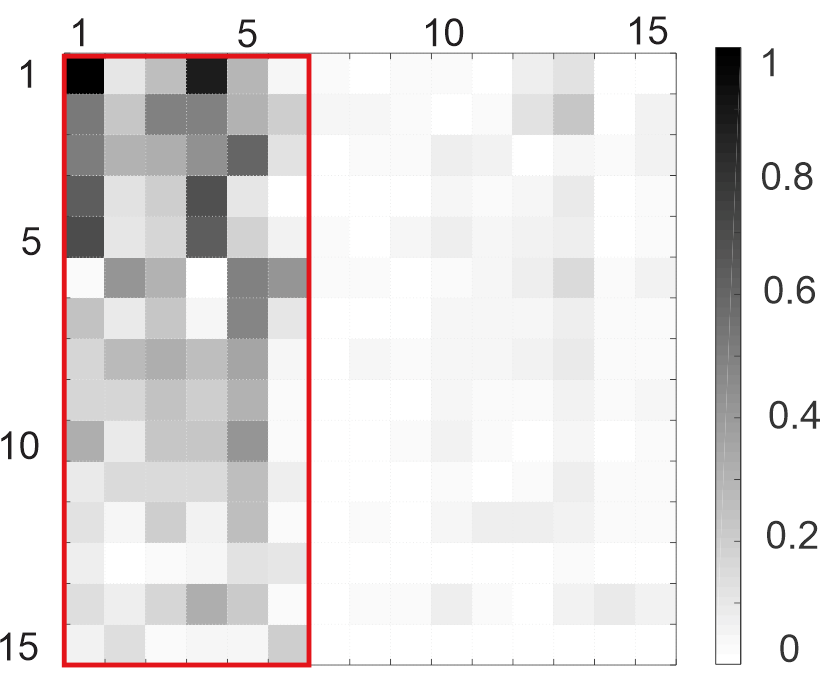
\includegraphics[width=0.85\columnwidth]{sparsity_ecg.png}
\caption{\textbf{The coefficients colormap of spatio-coupling matrix $A$. The distribution of normalized coefficients shows a subset of channels plays dominant roles in the cardiac dynamics. }}\label{fig:ECG_colormap}
\vskip -6mm
\end{figure}  

To verify the efficacy of our theoretical analysis results, we also consider the application of the algorithm to analyze the electrocardiogram (ECG). The raw clinical ECG data was extracted from the PTB diagnostic ECG database~\cite{goldberger2000physiobank}. Data on $52$ healthy subjects ($13$ women, age $48 \pm 19$ and $39$ men, age $42 \pm 14$) was obtained by the National Metrology Institute of Germany. Each subject's record includes 15 different signals simultaneously acquired: the conventional 12-lead (I, II, III, aV$_{\text{R}}$, aV$_{\text{L}}$, aV$_{\text{F}}$, V$_{\text{1}}$, V$_{\text{2}}$, V$_{\text{3}}$, V$_{\text{4}}$, V$_{\text{5}}$, and V$_{\text{6}}$) and 3 Frank orthogonal leads (V$_{\text{X}}$, V$_{\text{Y}}$, and V$_{\text{Z}}$). Each signal is digitalized at 1000Hz, with a signal bandwith of 0Hz to 1KHz and with 1 uV LSB resolution~\cite{Bousseljot1995}. As an example, we choose the ECG signal from the subject S0010 from the data set during a 39-second measurement session. Similarly, we first obtain the estimate of $\{\alpha_{j}\}$ that corresponds to the fractional order derivative in equation \eqref{fracDyn} and the spatio-coupling matrix $A$. Based on the identified system, the greedy algorithm shows we do not need more than two sensors(i.e., $I$ and $II$) to retrieve the dynamics of all 15-channel cardiac activities. We show the recovered system states using the observation from only two sensors in blue in Figure \ref{fig:ECG_exp}.(c-1). An important observation is that the obtained deployment of sensors aligns with the pattern distribution of coefficients in the coupling matrix $A$, see Figure \ref{fig:ECG_colormap}. A subset of channels plays the dominant role in the cardiac dynamics and these channels themselves are tightly coupled such that we can retrieve global dynamics by the observations made upon a subset of them. This is verified by the output of algorithm and validated during our simulation to generate the system states evolution at aV$_{\text{R}}$ as shown in Figure \ref{fig:exp_result}.(c-2). The simulated model response is strongly coherent with actual measurement. We set up the similar experiment to show the relation between the observation length and number of sensors deployed in context of a cardiac system. The results are shown in Figure \ref{fig:observ_ecg} and it is aligned with our previous observations made in the experiments of iEMG and EEG. The lower bound for the number of sensors used to reliably retrieve the global initial states can be identified by checking where the  phase-change appears. In the case of ECG, we notice there exists a sudden rise in the errors when only one sensor is considered. In contrast, we can achieve the similar accuracy if 2 or more sensors are placed in the measurement system as described in Figure \ref{fig:ECG_exp} given enough observations.

 \begin{figure}[htb]
\centering
\includegraphics[width=0.85\columnwidth]{observ_ecg.pdf}
\caption{\textbf{The accumulated errors are plotted against the length of observations and different settings of sensors. The longer observations improve upon the overall accuracy of system states estimates while it also suggests a lower bound for number of sensors used for observability. This observation aligns with our theoretical analysis on minimal observability. }}\label{fig:observ_ecg}
\vskip -4mm
\end{figure} 
\section{Summary}


Coupled-fractional dynamical systems capture the evolution of different physiological signals, such as electroencephalogram, electromyogram or electrocardiogram signals. In this paper, we proposed to determine the smallest collection of signals required to retrieve the overall evolution of the process modeled by the coupled-fractional dynamical system. In particular, we show that the problem is NP-hard, but a submodular approach  can be leveraged to obtain approximate solutions with optimality guarantees. Further, we illustrated the proposed mechanism in the context of the different mentioned physiological signals.
